\documentclass[tufte-handout]{standalone}
\usepackage{mathpazo} % Sets Palatino as the main font
\usepackage{tikz}
\usetikzlibrary{3d, angles, quotes, calc, backgrounds}
\usetikzlibrary{decorations.markings,shapes.geometric, arrows, positioning}

% my colors
\definecolor{darkslategray}{rgb}{0.18, 0.31, 0.31}
\definecolor{myorange}{rgb}{0.89804, 0.55686, 0.19608}

\tikzstyle{devel} = [ellipse, rounded corners, minimum width=1cm, minimum height=1cm,text centered, draw=black!90, thick, fill=darkslategray!0]
\tikzstyle{modules} = [rectangle, rounded corners, minimum width=3cm, minimum height=1cm, text centered, draw=darkslategray!85, fill=darkslategray!85]
\tikzstyle{output} = [rectangle, rounded corners, minimum width=3cm, minimum height=1cm, text centered, draw=darkslategray!30, fill=darkslategray!30]
\tikzstyle{decision} = [rectangle, rounded corners, minimum width=1.5cm, minimum height=1cm, text centered, draw=orange!30, fill=orange!30]
\tikzstyle{arrow} = [thick,->,>=stealth]
\tikzstyle{line} = [thick,-,>=stealth]

\begin{document}

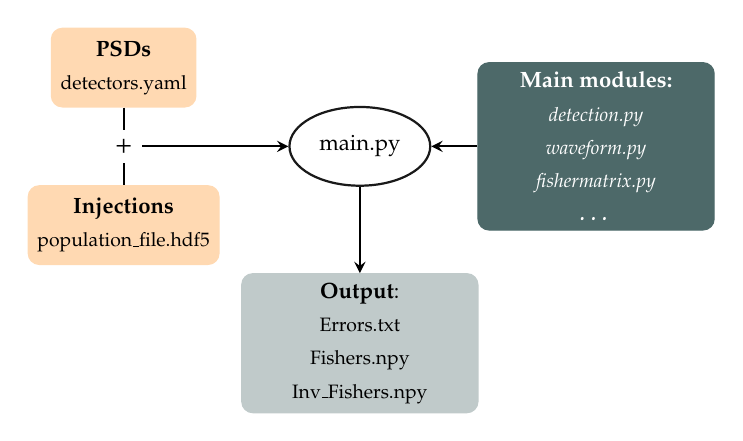
\begin{tikzpicture}[node distance=1.5cm, every node/.style={fill=white}, align=center]

% Main script
\node (main) [devel] {\footnotesize{main.py}};

\node (input1) [decision, left of=main, xshift=-1.5cm, yshift=-1cm] {\footnotesize{\bf{Injections} }\\\scriptsize{population\_file.hdf5}};
\node (input2) [decision, above of=input1, xshift=0cm, yshift = 0.5cm] {\footnotesize{\bf{PSDs}} \\\scriptsize{detectors.yaml}};

\node (modules) [modules, right of=main, xshift=1.5cm] {\textcolor{white}{\footnotesize{\bf Main modules:}}
\\\textcolor{white}{\textit{\scriptsize{detection.py}}}\\\textcolor{white}{\textit{\scriptsize{waveform.py}}} \\\textcolor{white}{\textit{\scriptsize{fishermatrix.py}}} \\\textcolor{white}{\textit{\dots}} };

\node (results) [output, below of =main, yshift=-1cm] { \footnotesize{\bf{Output}}:\\\scriptsize{Errors.txt} \\\scriptsize{Fishers.npy} \\\scriptsize{Inv\_Fishers.npy}};

\draw[line] (input2)  -- node (plus)[right of=input2, xshift = -1.5cm, execute at begin node = \setlength{\baselineskip}{0.42em}] {+} (input1);
\draw[arrow] (plus) -- (main);
\draw[arrow] (modules) -- (main);
\draw[arrow] (main) -- (results);

\end{tikzpicture}

\end{document}
